\section{Fundamentos de Machine Learning} \label{sec:anexo_fundamentos_machine_learning}

Este anexo resume conceptos de aprendizaje automático utilizados en la tesis, con énfasis en (i) el rol de las representaciones vectoriales (\textit{embeddings}) y (ii) el proceso de entrenamiento y evaluación de modelos.

\subsection{Jerarquía conceptual IA, ML y DL}

La Inteligencia Artificial (IA) es un campo de la informática que busca simular el comportamiento de la inteligencia humana, es decir, intenta replicar y automatizar la capacidad del ser humano para tomar decisiones.

Dentro del área de la Inteligencia Artificial, se encuentra el Machine Learning (ML), disciplina que a través del desarrollo de algoritmos y modelos busca que las máquinas aprendan patrones por medio de la experiencia, utilizando datos de entrenamiento y retroalimentación. El objetivo es entrenar un sistema para una tarea específica sin necesidad de programar explícitamente un conjunto de reglas para cada caso.

Finalmente, dentro de ML se encuentra el campo de Deep Learning (DL), un área que se centra en el uso de arquitecturas de redes neuronales profundas para aprender representaciones jerárquicas de los datos de forma automática \cite{deep-learning}.

\begin{figure}[h]
    \centering
    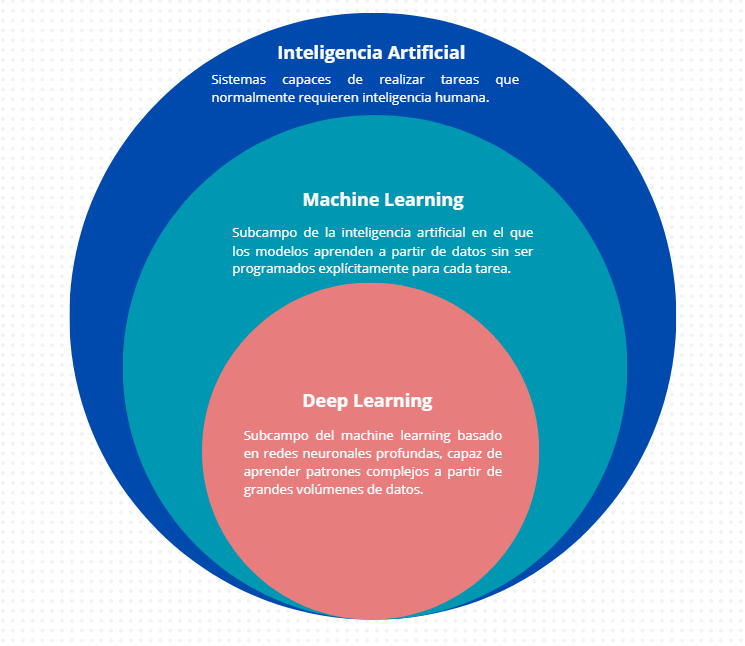
\includegraphics[width=0.75\textwidth]{Anexos/img/03/ia_ml_dl.png}
    \caption{Jerarquía conceptual entre Inteligencia Artificial, Machine Learning y Deep Learning.}
    \label{fig:ia_ml_dl_jerarquia}
\end{figure}

\subsection{Conceptos básicos de aprendizaje automático}

\subsubsection{Tipos de aprendizaje y tareas}

En términos generales, los problemas de aprendizaje se pueden agrupar en:
\begin{itemize}
    \item \textbf{Aprendizaje supervisado}: se cuenta con pares $(x_i,y_i)$, donde $x_i$ representa la entrada (atributos) y $y_i$ la etiqueta objetivo. El modelo aprende una función $f_\theta$ que aproxima $y$ a partir de $x$. Tareas típicas son clasificación y regresión.
    \item \textbf{Aprendizaje no supervisado}: no se dispone de etiquetas; se busca descubrir estructura en los datos (por ejemplo, agrupamiento o reducción de dimensionalidad).
    \item \textbf{Aprendizaje auto-supervisado}: se construyen objetivos a partir de los mismos datos para aprender representaciones útiles sin etiquetas explícitas (por ejemplo, predecir partes faltantes, contexto o transformaciones).
\end{itemize}

En esta tesis, el objetivo principal se relaciona con tareas supervisadas (por ejemplo, clasificación de relaciones económicas entre ASes) y con aprendizaje de representaciones, donde la calidad del \textit{embedding} impacta directamente el desempeño del modelo final.

\subsubsection{Representaciones y \textit{embeddings}}

Una \textbf{representación} corresponde a una codificación de una entidad (por ejemplo, un AS) en una forma que pueda ser procesada por un modelo. En ML, una representación común es un vector numérico $x\in\mathbb{R}^d$ que reúne atributos o descriptores.

Un \textbf{\textit{embedding}} es una representación vectorial densa (de dimensión relativamente baja) que se aprende o construye con el objetivo de preservar información relevante sobre la entidad y su contexto. A diferencia de codificaciones dispersas como \textit{one-hot}, los \textit{embeddings} permiten capturar nociones de similitud: entidades con roles o contextos similares tienden a quedar cercanas en el espacio vectorial.

En el contexto de esta tesis, las representaciones pueden provenir de:
\begin{itemize}
    \item \textbf{Atributos tabulares}: características extraídas desde fuentes como PeeringDB (por ejemplo, tipo de red, políticas, presencia en IXPs).
    \item \textbf{Estructura de conectividad}: representaciones derivadas de rutas BGP o de la topología del grafo, donde el ``contexto'' de un AS está determinado por su vecindad o por sus co-ocurrencias en caminos.
\end{itemize}

\subsubsection{Entrenamiento, validación y evaluación}

En un flujo estándar de aprendizaje supervisado, los datos se separan en conjuntos de \textbf{entrenamiento}, \textbf{validación} y \textbf{prueba}. El entrenamiento ajusta parámetros $\theta$ minimizando una función de pérdida $L(\theta)$ (por ejemplo, entropía cruzada para clasificación), típicamente mediante variantes de descenso por gradiente (por ejemplo, SGD o Adam).

El conjunto de validación se utiliza para seleccionar hiperparámetros (dimensión del \textit{embedding}, tasa de aprendizaje, número de épocas, regularización, etc.) y controlar \textit{overfitting} mediante estrategias como \textbf{early stopping}. El conjunto de prueba se reserva para reportar desempeño final.

En problemas con \textbf{desbalance de clases}, es importante complementar métricas globales (por ejemplo, \textit{accuracy}) con métricas por clase o promediadas (por ejemplo, \textit{precision}, \textit{recall} y $F_1$), y considerar técnicas como ponderación de la pérdida o muestreo estratificado para evitar modelos sesgados hacia la clase mayoritaria.

\subsection{Arquitecturas neuronales clásicas (FFNN, RNN, CNN)}

\subsubsection{Redes Neuronales Feed Forward (FFNN)}

También conocidas como \textit{multilayer perceptrons}, estas arquitecturas representan la forma más simple y fundamental de una red neuronal, sirviendo como base de múltiples modelos de Deep Learning. En esta arquitectura la información fluye exclusivamente hacia ``adelante'', sin bucles o conexiones recurrentes.

El flujo comienza en la capa de entrada, seguida de capas ocultas (típicamente \textit{fully connected}), donde cada neurona se conecta con las neuronas de la capa anterior. El objetivo general es aproximar una función $f(x)$; por ejemplo, en regresión se busca modelar una relación $y=f(x)$.

\subsubsection{Redes Neuronales Recurrentes (RNN)}

Las redes neuronales recurrentes (RNN) son una variante de redes \textit{feed forward} con capacidad de incorporar información previa, es decir, poseen ``memoria''. A diferencia de las FFNN, las RNN introducen conexiones desde estados anteriores hacia el estado actual, lo que permite modelar dependencias temporales.

Esta característica hace a las RNN adecuadas para trabajar con datos secuenciales, como procesamiento de lenguaje natural y predicción de series temporales.

\subsubsection{Redes Neuronales Convolucionales (CNN)}

Las redes neuronales convolucionales (CNN) son un tipo especializado de modelo diseñado para procesar datos con estructura de grilla (por ejemplo, imágenes). Estas redes aplican operaciones de convolución mediante filtros (kernels) que aprenden patrones locales (bordes, texturas, formas), combinándolos jerárquicamente a través de múltiples capas.

Estas arquitecturas ilustran por qué, para datos relacionales de tipo grafo, es necesario incorporar explícitamente la estructura de conectividad; esto motiva el uso de Redes Neuronales de Grafos (GNNs), descritas en el anexo siguiente.

